\chapter{Features and Metrics}
\label{chp:b3}

In this thesis, image representations and the scheme that these representations are related constitutes the basics of the assessment of similarity between images. In this chapter, first, image features that are used to represent images are presented. The image features measure different aspects of the image and also differ in representation. Therefore, the metrics that estimate the distance between image features need to be chosen accordingly. Several distance metrics are presented in the second part of this chapter and for each feature the selected distance metric is given. 

\section{Image Features}
\label{sec:features}
As the most fundamental part of many computer vision applications, image feature extraction is a widely studied research topic for the last several decades. There are numerous image features in the literature developed with different purposes which can be divided into two broad categories: global and local features. While global features like histograms of image properties represent the whole image with a single feature vector, local features like SIFT~\cite{lowe2004distinctive} or SURF~\cite{bay2006surf} are a collection of vectors representing small neighborhoods called interest regions. Although local features are used successfully for the applications like image classification or retrieval, this thesis focuses on global features to investigate the image similarity in a general sense. In this section, a review of global image features that have been used in this thesis is given. Table~\ref{tab:table_feature} lists these features together with their representations and the distance metric used for each feature. 

\begin{table}
\caption{HDR Image features and distances}
\centering
\begin{tabular}{c|c|c}
\label{tab:table_feature}
\textbf{Feature} & \textbf{Model} & \textbf{Distance Metric}\\
\hline
Color  & 2D chromaticity histogram & EMD \\
Luminance  & 1D (relative) luminance histogram & EMD \\
Texture  & Histograms of gradients & EMD \\
GIST  & Feature vector & Cosine distance \\
VGG16/VGG19 - fc6 & Fused fc6 layer & Cosine distance  \\
VGG16/VGG19 - fc7 & Fused fc7 layer & Cosine distance
\end{tabular}
\end{table}

%paper
\subsection{Color}
%paper
Since the early days of the image similarity research, color has been used as one of the most discriminative cues~\cite{neumann2006image}. In this thesis,  we used the $a$ and $b$ channels of the CIELAB color space~\cite{iso201111664} to represent chromaticity information. This is an opponent color space, where the $a$ channel represents red/green opponent colors and the $b$ channel yellow/blue opponent colors. We used a 2D chromaticity histogram to represent the distribution of colors in a given image. Each dimension contained $15$ bins for a total of $225$ bins. Figure~\ref{fig:hists} shows this histogram for the Mason Lake image from the dataset~\cite{fairchild2007hdr}.

\begin{figure}
\centering
\begin{tabular}{c c}
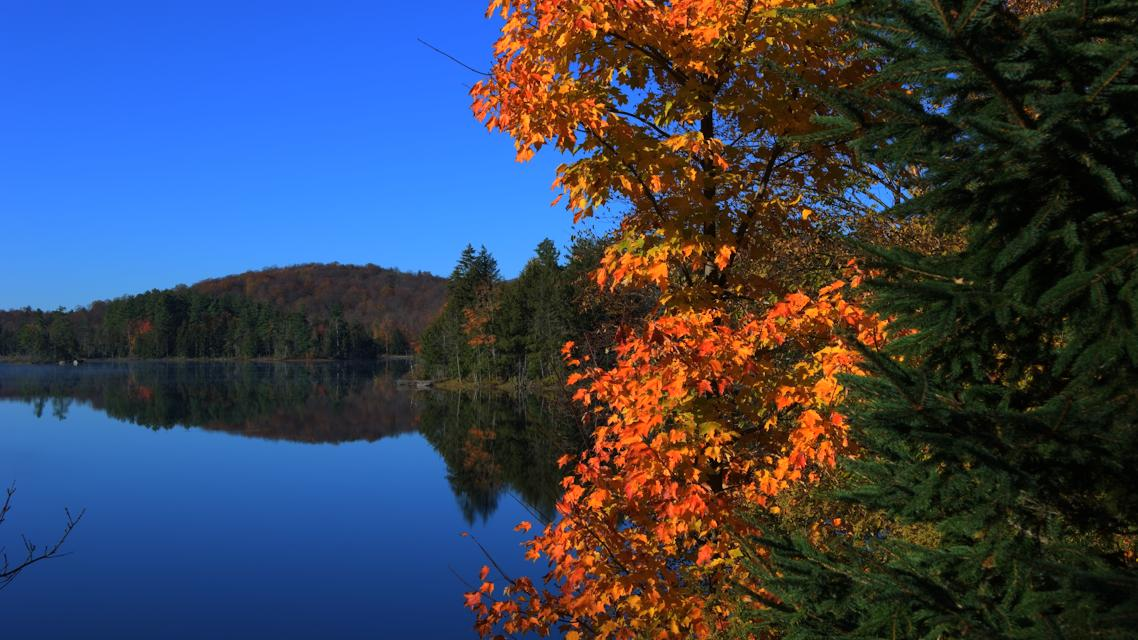
\includegraphics[height=1.8in]{figures/chapter2/MasonLake.jpg} &
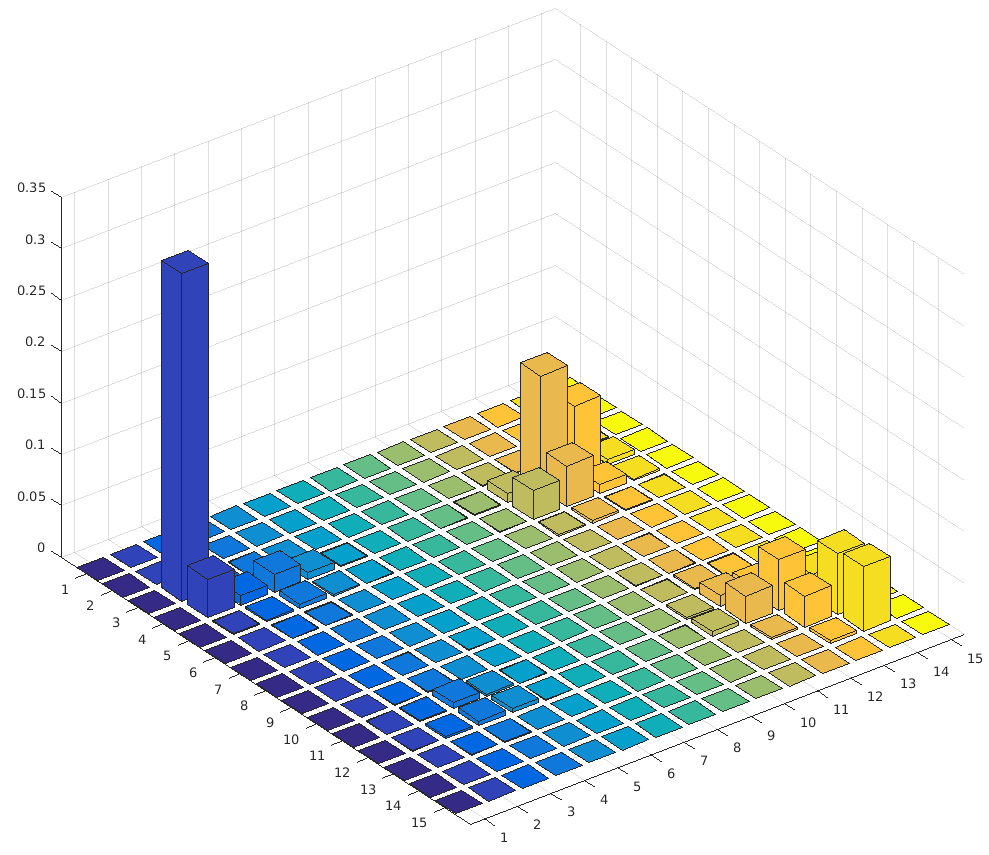
\includegraphics[height=1.8in]{figures/chapter2/57_histab.png}
\end{tabular}
\caption{Sample image (left), 2D histogram (right).}
\label{fig:hists}
\end{figure}

%paper
\subsection{Texture}
%paper
Texture is the second most used feature for content based image retrieval systems after chromatic features. This feature is especially helpful for discriminating images that have similar color but different spatial characteristics such as blue sky and sea or sand and buildings. In this thesis, to represent the texture information histogram of gradient magnitudes~\cite{sharma2015histogram} is used. 
%paper
\subsection{Luminance}
%paper
The main difference between an HDR and an LDR image is the much wider range of luminance distribution for the former. A single HDR image may contain very low luminances corresponding to highly shadowed regions as well as very high luminances corresponding to bright highlights. Therefore, we hypothesized that the luminance distribution of an HDR image may be an important cue for visual similarity. The luminance distribution is modeled using a 1D (relative) luminance histogram with $50$ bins.
%paper
\subsection{GIST Features}
%paper
The GIST descriptor~\cite{oliva2001modeling} aims to represent the dominant spatial structure of a scene by using low level multi-scale representations. This descriptor defines the scene as a whole rather than focusing on individual objects or regions. Discriminative properties of a scene are listed as naturalness, openness, roughness, expansion, and ruggedness. The class of a scene, e.g., man-made, natural, indoor, outdoor, etc., is determined by these properties.

The procedure for extracting GIST descriptors consists of applying Gabor filters that are scaled and orientated differently to the input image, dividing the filter response map into a grid in order to have spatial information, averaging the filter response in each grid, and concatenating the results to obtain the final feature vector, i.e. the GIST descriptor.

%paper
\subsection{Deeply Learned Features}
%paper
Recently, DCNNs have started to dominate object recognition and image classification tasks, achieving near human success rates~\cite{krizhevsky2012imagenet,simonyan2014very,zhou2017scene}. These models are trained with large prelabeled datasets and develop a hierarchical model that becomes more aware of the content of the image rather than the underlying pixel values. To our knowledge currently there is no DCNN model that is trained on HDR images for the purpose of image indexing, scene classification, or visual similarity tasks.
Furthermore, there is no prelabeled large HDR image dataset to use for training a DCNN model from scratch. Therefore in this thesis, we used transfer learning method to employ pretrained DCNNs for our perceptual similarity problem. 

For feature extraction, pretrained AlexNet~\cite{krizhevsky2012imagenet} and two variants of VGG networks, VGG16 and VGG19, are used~\cite{simonyan2014very}. All networks are trained on the ImageNet~\cite{russakovsky2015imagenet} dataset, but we also evaluated their performance when trained using different datasets. For transfer learning, the last fully connected layer, which contains classification outputs, is removed and the remaining $4096$ dimensional two fully connected layers, \textbf{fc6} and \textbf{fc7}, are used as feature vectors. As suggested by Simonyan and Zisserman~\cite{simonyan2014very}, the results obtained from VGG16 and VGG19 are fused (by taking an average) and it is observed that the fused version performs better than both VGG16 and VGG19. The distance between the feature vectors are calculated using cosine distance, which is a commonly used distance metric for deep learning features. 

%\section{Computational Complexity}
%A brief analysis of computational complexity of the features is provided in this section. The color and luminance features are merely histograms and they can be computed in O(N) time, where N represents the number of image pixels. The GIST descriptor is based on computing the convolution of 32 Gabor filters at 4 scales and 8 orientations to compute feature maps and then averaging the features to obtain a 16 element vector per feature map. These vectors are then concatenated to find the final feature vector. Therefore, the GIST feature also has a linear time computational complexity. The texture feature represented by HOG is similar to GIST in terms of its operation, albeit being somewhat simpler, and also has a linear complexity. Finally, the deeply learned features are computed by a single forward application of the VGG network, which also involves several convolutions at multiple scales as well as application of activation functions. As the convolutional kernel sizes are negligible compared to the image size, the computation of VGG features also has a linear time computational complexity. In summary, all of the features can be computed at real-time rates in modern hardware, especially if GPUs are utilized.
%paper
\section{Distance Metrics}
%paper
The use of a proper distance metric is as important as the features themselves. Each feature representation
may require a different distance metric. In this section, we briefly describe the definitions and properties of the dissimilarity measures that we used for different types of features.
%paper
\subsection{Euclidean Distance}
%paper
The Euclidean distance between two histograms p and q is calculated as:
\begin{equation}
dist_{euc}(p,q) = \sqrt{\sum_i(p_i-q_i)^2},
\end{equation}
where i is the bin index. In general, dissimilarity obtained by Euclidean distance for histograms is not satisfactory as it does not take bin proximity into account.
%paper
\subsection{Bhattacharyya Distance}
%paper
Bhattacharyya distance~\cite{bhattacharyya1946measure} measures the overlap between two distributions. If p and q are two histograms, it can be calculated as:
\begin{equation}
dist_{bhat}(p,q) = -\ln \left( \sum_i \sqrt{p_i.q_i} \right).
\end{equation}

For our HDR similarity problem Bhattacharyya distance gives slightly better results than Euclidean distance. However, it also suffers from the same problem that the proximity of the bins is not taken into account.
%paper
\subsection{Earth Mover’s Distance}
%paper
Earth Mover’s Distance (EMD) is a dissimilarity metric commonly used for image the retrieval problems~\cite{rubner2000earth}. EMD aims to capture the perceptual similarity between two distributions by calculating the minimal cost of transforming one distribution to the other. Unlike the other dissimilarity metrics, EMD can be calculated for varying-size partitions of the data, called signatures.
Signatures consist of dominant clusters of the data, represented as $si = (m_i, w_i)$ pairs where mi is the cluster center and $w_i$ is the size of the cluster. EMD does not require the signatures to have the same number of clusters – ground distances between cluster centers are sufficient. Histograms are signatures with bin centers corresponding to cluster centers, mi, and normalized bin values to weights, $w_i$.

The total amount of work to transform distribution
p to q with flow f is:
\begin{equation}
WORK(P,Q,F) = \sum_i^m \sum_j^n d_{ij}f_{ij}, 
\end{equation}
where dij is the ground distance between cluster centers i and j. The optimal flow f that results with the minimum work, can be found by any linear optimization algorithm. When f is calculated, the EMD between p and q is defined as:
\begin{equation}
EMD(p,q) = {{\sum \sum d_{ij}f_{ij}}\over{\sum \sum f_{ij}}}.
\end{equation}
In our problem, bin centers correspond to color values (ab values in the CIELAB space) and ground distances are calculated as Euclidean because of the perceptual uniformity of the CIELAB color space.

Figure \ref{fig:sim_comp} compares the effect of these three distance metrics for a sample image from the dataset. The image on the first column is the query image, and in each row, the most similar five images from the dataset are shown. The distance metric used in first row is Euclidean, the second row is Bhattacharyya, and the last row is the EMD. It can be argued that more similar images are found using the EMD metric.

\begin{figure} 
\centering
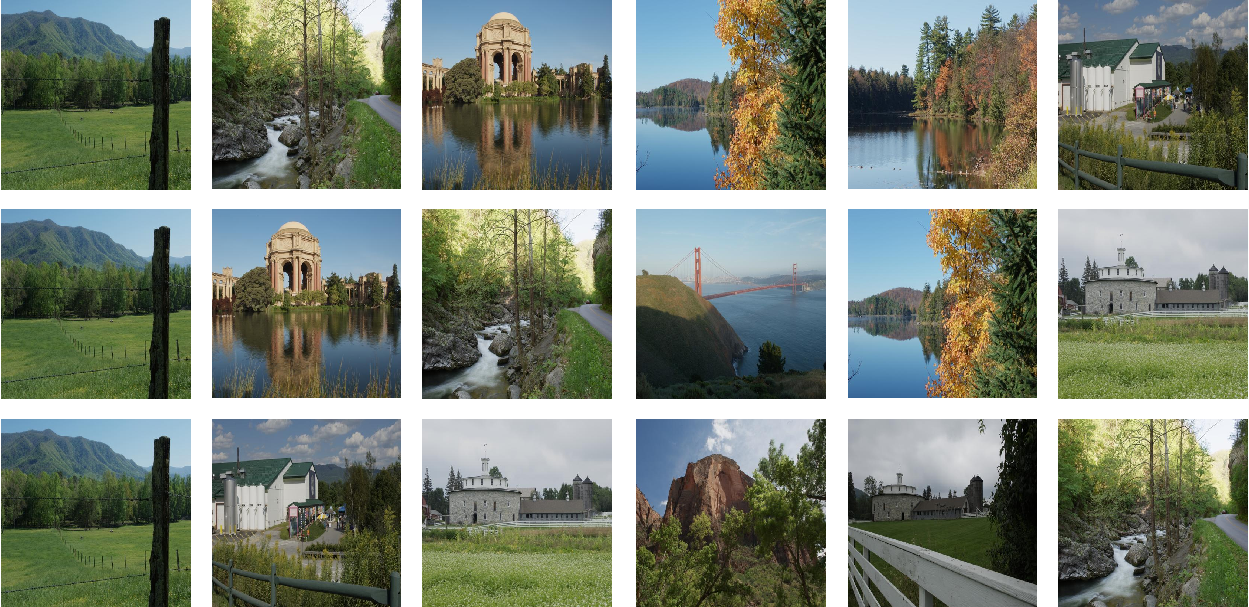
\includegraphics[width=\textwidth]{figures/chapter2/16sims.png}
\vspace{10pt}
\caption{A comparison of dissimilarity metrics for histogram-based features. The leftmost image is the query image, the most similar five images from the dataset are shown in each row: Euclidean distance (first row), Bhattacharyya distance (second row), Earth Mover’s distance (third row).}
\label{fig:sim_comp}
\end{figure}

%paper
\subsection{Cosine Similarity}
%paper
Cosine distance between two vectors $p$ and $q$ is calculated as:
\begin{equation}
dist_{cosine}(p,q) = 1 - {{\sum_{i=1}^{n}p_{i}q_{i}} \over {\sqrt{\sum_{i=1}^{n}p_{i}^2}} \sqrt{\sum_{i=1}^{n}q_{i}^2}} 
\end{equation}
Cosine distance is a widely used distance metric for deep representations. In this thesis, we used cosine distance for calculating the distances between CNN feature vectors and GIST features.